In the previous section, we identified certain limitations in the current offloading strategies
in the COMET infrastructure. To address them we devised certain heuristics based on our analysis
of android applications.

\subsection{Parent-to-Native Execution Time}
Currently, COMET identifies a set of native methods that can be offloaded. These methods are annotated manually
and the run-time system determines if the current native method can be flagged as offloadable. This is done for
approximately 200 native methods. In addition to these methods, the application has many other native function calls
that cannot run on the server. The current offload infrastructure will abort execution at the server and invoke a sync
call to send the state back to the client. This process of sending state from client to server and receiving state on
aborting at native call can be very expensive, especially with limited network bandwidth.

We address this issue by profiling the application by obtaining the execution time betweeen the each parent method and its
first native method invocation. If this execution time is very small as compared to the time required to send the data during
a sync operation, then it would be unadvisable to perform a sync at the parent method and send the state to the server. By marking the parent as
unsafe to offload, we avoid the sync time in sending and receiving data when the application aborts at the server.
Figure~\ref{fig:parent_native} shows an example of a parent method Pa and its native method Na. t1 denotes the end of Pa and t2
denotes the start of the native method Na. The time duration $t2-t1$ includes the non-native execution code. We can compare this
time difference with the last sync time (or get the sync time based on current bandwidth and data transfer size)

%-------------------------------------------------------%
\begin{figure} [thf*]
\centering
\begin{tabular}{c}
\begin{minipage}[b]{0.5\textwidth}
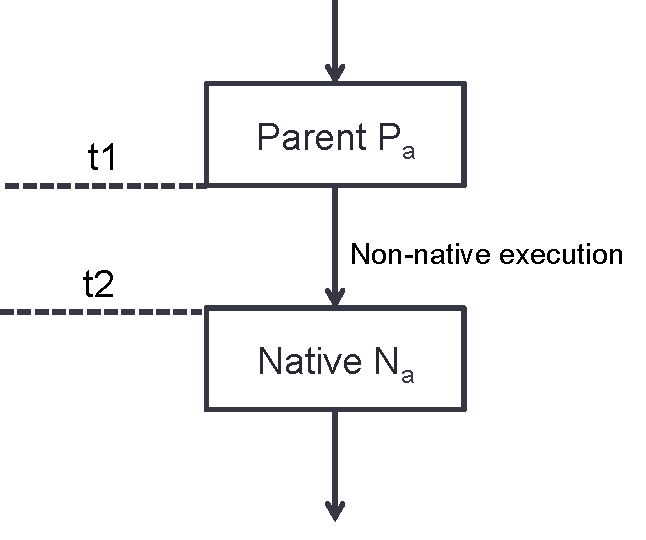
\includegraphics[width=0.95\textwidth]{figs/parent_native.pdf}
\end{minipage}
\end{tabular}
\caption{Call Graph with Parent and Native method having non-native execution time $t2-t1$}
\label{fig:parent_native}
\end{figure}
%-------------------------------------------------------%
\subsection{Native-to-NextNative Execution Time}
The offloading strategy that COMET currently implements is a simple one. It looks at the value of the Round Trip Time (RTT) and
the Sync Time to calculate a threshold. The offloading is enabled if this threshold is less than the time elapsed since the last
time an abort was invoked at the server. This strategy might not exploit the offloading capabilities to the fullest as it waits for
some time before deciding to migrate to the server.

Our analysis on applications revealed that certain applications have a huge chunk of non-native execution code that is computationally
intensive after a native function call. Even a simple application that invokes the client-side display periodically and has a lot of intense
computation between these native calls will get affected to some extent by this mechanism. Our static analysis also reveals that significant
amount of time is spent in non-native execution between two native calls. In such a scenario, we offload immediately after the first
native method returns to the client. With the profiling results, we can isolate the computationally intensive portions of code that
are of interest to us and set a flag to inform the scheduler to perform migration without waiting to cross a threshold. The scenario
mentioned is shown in Figure~\ref{fig:native_native}. In this figure the time difference $t3-t2$ is of interest to us as it denotes the amount
of non-native execution that can execute on the server. If the profiling results suggest that this time difference is significant, then we
inform the COMET scheduler to migrate to the server after executing the Native method Na locally.

%-------------------------------------------------------%
\begin{figure} [thf*]
\centering
\begin{tabular}{c}
\begin{minipage}[b]{0.5\textwidth}
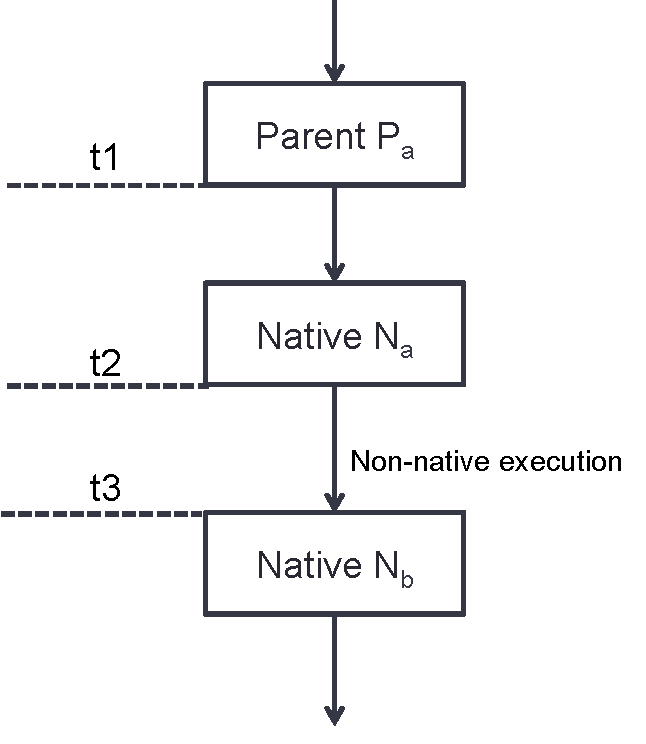
\includegraphics[width=0.95\textwidth]{figs/native_native.pdf}
\end{minipage}
\end{tabular}
\caption{Call Graph with non-native execution time $t3-t2$}
\label{fig:native_native}
\end{figure}
%-------------------------------------------------------%

\subsection{Bandwidth Check}
COMET relies on good netowrk conditions to ensure that the synchronization operations between client and server occur with less overhead. Infact as detailed in Section \ref{motiv}, the scheduling decision is based on the time it took for the last synchronization which is affected to a certain extent by the available bandwidth. Studying the current implementation of COMET we noticed that though the last sync time is considered in decision making, the size of data to be transferred was not being considered. We wanted to better the decision making by migrating a thread only when the data size to be transferred was lesser than a threshold that was derived based on current bandwidth conditions. Our idea was that even though the latest sync time can be huge, if the time it takes to migrate the data is lesser than the time it takes to run on the client, it is better to migrate that thread at that point. We discuss the implementation and evaluation of our ideas in the respective sections. 
